\subsection*{Functional closure as an invariant property of evolvable systems}

In this section, we will attempt to explain the functional closure property in category theoretic terms. The abstract components have been related to biological ones in the previous section. The biological property from which Rosen derived his diagram expressing the functional closure concept is metabolism regarded in the manner described above and as depicted in Figure \ref{fig:metabolicstringdiag}. A metabolic mapping in an evolvable system $\mathcal{E}$ can be thought of as a morphism between two objects in $\mathcal{E}$, the latter now regarded as an abstract algebraic category:
\begin{align*}
f \colon A &\longrightarrow B\\
a &\longmapsto f(a)=b
\end{align*}

In category theory, we can imagine the abstract objects and morphisms as specializing to a particular type of algebraic structure and, thus, as a first approximation we can think of both objects as (cartesian product) sets, where $A$ represents a configuration of input substrates and $B$ likewise for metabolite products of metabolic transformations such as $f$. This abstraction of some aspects of an evolvable system could be further developed by substituting more highly structured objects than sets that meet intuitive and otherwise empirically suggested features of evolvable systems. We can consider all such \emph{metabolisms} together as the set of all the different morphisms between these objects referred to, if such an object exists at all, as the \emph{internal} exponential object $B^A$ \footnote{see Materials and Methods for the precise definition of exponetial object} or the \emph{external} hom-set $Mor_{\mathcal{E}}(A,B)$.

The apparently finite nature of evolvable systems, imposes several constraints regarding the maintenance of sufficient concentrations of the components that constitute it. As enzymes necessary for metabolism decay, they must be regenerated, from the metabolic products, or the system comprised of them will disintegrate. In addition, fluctuations in the substrates $A$ have to be corrected by the differential availability and performance of the overall metabolic morphism $f$. Hence, there must be a collection of morphisms from $B$ to $B^A$, one of which can be identified with the information required to \emph{regenerate} the enzymes necessary for core metabolic processes:
\begin{align*}
g \colon B &\longrightarrow B^A\\
b &\longmapsto g(b)=f
\end{align*}
This \emph{regeneration} system itself represented by $g \in B^{A^B}$ is also assumed to have a finite lifetime and thus requires a form of \emph{meta-regeneration} by some other system:
\begin{align*}
h \colon B^A & \longrightarrow B^{A^B}\\
f & \longmapsto h(f)=g.
\end{align*}	
In the biological metaphor commonly associated to this abstract construction, this \emph{meta-regeneration} system is associated either to the maintenance of some degree of structural invariance in the topology of the combined gene regulatory and metabolic interaction networks underlying an organism. In this light, this process may be associated to the DNA replication and reproduction process. In any case, the argument proliferating hierarchical levels of organization necessary to strive toward functional closure may be continued \emph{ad infinitum} (i.e. the next step would be to ask for the origin of $h$ and to posit the existence of another higher-order morphism that takes $g$ as input and produces $h$, see Figure \ref{fig:hom}b). 

From a biological perspective, systems of the form described may be able to avoid such an infinite regress by achieving a form of \emph{functional closure} in which, for example, we can materially identify a metabolic product $B$ with a replication function $h$ or perhaps even with the entire set of replication functions $B^{A^B{^B{^A}}}$. If we take the former case then we have introduced a problem that cannot be dealt with given the definition of a category because of the fundamental typing distinction therein between objects and morphisms. Although we might be able to associate an element or point of the object or type $B$ with $h \in B^{A^B{^B{^A}}}$, we sustain a typing error if we attempt to express the fact that these are materially equivalent because $h \colon 1 \rightarrow B$ is of type $B$ while $h \colon B^A \rightarrow B^{A^B}$ is of type $B^{A^B{^B{^A}}}$. Thus we would attempt to state $h:B = h:B^{A^B{^B{^A}}}$, but this is impossible to do, at least naively, within category theory as it produces a type error due to the fact that equations are only allowed between elements (respectively paths) with the same type (respectively with the same domain and codomain) Figure \ref{fig:hom}a. The other option is to avoid attempting to identify such elements and attempt to simply identify objects themselves. In this sense, we would attempt to express closure internally as $B \cong B^{A^B{^B{^A}}}$ or externally as $Mor_{\mathcal{E}}(1,B) \cong Mor_{\mathcal{E}}(B^A,B^{A^B})$. This approach could be considered to solve the typing issue since we could more explicitly state that $B \colon Set \cong B^{A^B{^B{^A}}} \colon Set$ or more generally for any category $B \colon Ob(\mathcal{E}) \cong B^{A^B{^B{^A}}} \colon Ob(\mathcal{E})$. However, we have now implied something stronger and less intuitive about the biological meaning of functional closure by stating that the set of metabolites is somehow isomorphic to the set of \emph{all possible} replication morphisms. Moreover, if such a relationship were to be satisfied, it could only be satisfied by the most trivial case in the category of sets $A = \{*\} = B$ so that $|B|=1=|B^{A^B{^B{^A}}}|$.

We have not yet attempted to make explicit how it might be possible to perform the identification between an element of type $B$ and another of type $B^{A^B{^B{^A}}}$ as expressed in Figure \ref{fig:hom}c. The original argument describing functional closure in a sense settles for stating something weaker than what we have already suggested is impossible to do directly within category theory (i.e. to state for some $h$, $h:B = h:B^{A^B{^B{^A}}}$). The most important feature of this argument is the concept of an evaluation map (see Materials and Methods) or morphism, which is intrinsic to the definition of exponential objects and thus evaluation maps exist in categories, like the primary example of the category of $\mathbf{Sets}$ we have considered thus far, having exponential objects. Given a category with products and exponentials, the evaluation map can be curried (i.e. in this case a function of two variables that returns a value can be converted to a function of one variable that returns a function) in the following manner
\begin{prooftree}
				\AxiomC{$B^{A} \times A \xrightarrow[]{ev} B$}
				\UnaryInfC{$A \xrightarrow[]{\hat{ev}} B^{B^A}$}
\end{prooftree}
where the maps $\hat{ev}$ are defined pointwise as
\begin{align*}
\hat{ev}(a) \equiv ev_a \colon B^A &\longrightarrow B,\\
f &\longmapsto ev(f,a) = f(a).
\end{align*}
This construction can be applied analogously at the next level regarding the evaluation of functions of the type $B^{A^B}$, by applying them to arguments of type $B$, to functions of the type $B^A$. The currying of the evaluation map is given by
\begin{prooftree}
				\AxiomC{$B^{A^B} \times B \xrightarrow[]{ev} B^A$}
				\UnaryInfC{$B \xrightarrow[]{\hat{ev}} B^{A^{B^{A^B}}}$}
\end{prooftree}
where the maps $\hat{ev}$ are defined pointwise as
\begin{align*}
\hat{ev}(b) \equiv ev_b \colon B^{A^B} &\longrightarrow B^A,\\
g &\longmapsto ev(g,b) = g(b).
\end{align*}
Although the continuation of the functional closure argument may also be applied in the first case of $ev_a$, we will apply it to the next level involving $ev_b$ to maintain the intuitive property that the metabolic substrate configuration represented by $A$ also represents material being extracted from the environment while functional closure is assumed to be achieved internal to the metabolic network (represented by $f$) and the regulatory apparatus (represented by $g$ and $h$) layered on top of it despite the material connection via $A$ to the environment.

We first consider the preimages of the evaluation morphisms as
\begin{align*}
\hat{ev}^{*}(b) \equiv ev^{*}_b \colon B^A &\longrightarrow B^{A^B},\\
f &\longmapsto g |g(b)=f.
\end{align*}
If, in this case, the evaluation morphism can be shown to have an inverse (i.e. $\hat{ev}^{*} \circ \hat{ev} = 1_A$ and $\hat{ev} \circ \hat{ev}^{*}= 1_{B^{B^A}}$) for some potentially restricted domain of definition of $\hat{ev}$ then the inverse morphism can also be defined pointwise as 
\begin{align*}
\hat{ev}^{-1}(b) \equiv ev^{-1}_b \colon B^A &\longrightarrow B^{A^B},\\
f &\longmapsto g | g(b) = f.
\end{align*}
In this sense, if there is a unique $g$ satisfying $g(b)=f$ for each combination of $b$ and $f$ in the restricted domains of definition then $b$ and $f$ can be viewed as determining $g$. This relieves what otherwise appears to be the necessity of positing the existence of an $h$ to answer the question of the origin of $g$. This is the weaker statement that is supported by this argument as compared to the stronger version, which could ostensibly be expressed as $b:B = h:B^{A^{B^{B^A}}}$.

\begin{figure}
\begin{center}
\noindent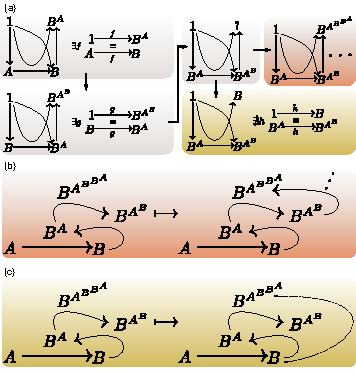
\includegraphics[width=0.75\columnwidth]{fig/mrcatclosure.pdf}
%\noindent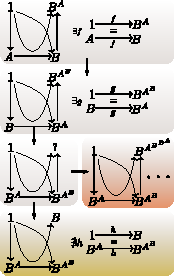
\includegraphics[width=0.24\columnwidth]{fig/mrcatprob.pdf}
\end{center}
\caption{Rosen's diagram attempting a depiction of functional closure in a cartesian closed category. (a) The top-left panel shows the identification of morphisms with domain $A$ and codomain $B$ with elements of the exponential object $B^A$. The bottom-left panel shows the analogous relationship between morphisms with domain $B$ and codomain $B^A$ and the exponential object $B^{A^B}$. On the right, two alternatives are shown in the last step. Either one can (b) continue on the path leading to infinite regress or (c) take the path leading to immediate closure.}
\label{fig:hom}
\end{figure}

\subsection*{Functional closure expressed in a type-free setting}
This argument describing functional closure so far suggests constraints by which we may be able to \emph{determine} some $h$ via $b$ (and also $f$), but so long as the ultimate goal is to state that for some $b$, $b:B = h:B^{A^B{^B{^A}}}$, it appears that it cannot be done in an obvious way in category theoretic terms. This is a result of the typing discipline inherent to the category theoretic description used thus far. We will ultimately find that we can re-express a stronger form of the functional closure in category theoretic terms, but in a manner that it is not obvious how to define directly within category theory. We thus first re-consider the expression of functional closure in terms of another language, the lambda calculus, which has both type-free and varying degrees of typed forms \cite{Barendregt1985} before returning to the so-called categorical semantics that enable the re-expression of this stronger form of functional closure in category theoretic terms.

If we reconsider the discussion in the previous section without regard for any typing discipline, we can summarize the proliferation of levels of organization up through the first three discussed in the following system of equations
\begin{align*}
f(a)&=b,\\
g(b)&=f,\\
h(f)&=g.
\end{align*}
It is trivial to express the functional closure property so long as we are able to disregard any typing discipline by identifying $h$ with $b$. In this case we can express functional closure as
\begin{align*}
f(a)&=b,\\
g(b)&=f,\\
b(f)&=g.
\end{align*}

%In order for  $\mathcal{E}$ to be functionally closed every morphism must be represented by or be in turn an object of the category. As we have stated, the set of functions $Mor_{\mathcal{E}}(A,B)$ between two objects in the category can be represented by the exponential object $B^A$. These exponential objects are associated with so-called evaluation maps both for the metabolic morphisms:
%\begin{align*}
%e_f : B^A \times A &\longrightarrow B,\\
%(f,a) & \longmapsto f(a),
%\end{align*}
%and for the maintenance system:
%\begin{align*}
%			e_g: B^{A^B} \times B &\longrightarrow B^A,\\
%	    			            (g,b) & \longmapsto    g(b).
%\end{align*}		
%We can take the system as described and develop all the exponentiations of its maps and represent all the evaluation functions of its exponential objects:		
%$$
%			\xymatrix{
%			 ... & ... & ... \\
%			  B^{A^{B^A}} \times A \ar[r]_-{\epsilon} \ar[u]^-{..^A} & B^{A^B} \ar[u]^-{..} & B^{A^{B^B}} \times B\ar[l]^-{\epsilon}\ar[u]^-{..^B} \\
%			 B^{A^A} \times A \ar[r]_-{\epsilon} \ar[u]^-{r^A} & B^A \ar[u]^-{r} & B^{A^B} \times B\ar[l]^-{\epsilon}\ar[u]^-{r^B} \\
%			B^A \times A \ar[r]_-{\epsilon} \ar[u]^-{g^A} & B \ar[u]^-{g} & B^B \times B\ar[l]^-{\epsilon}\ar[u]^-{g^B} \\
%			A^A \times A \ar[r]_-{\epsilon} \ar[u]^-{f^A} & 
%			A\ar[u]^-{f} & A^B\times B\ar[l]^-{\epsilon}\ar[u]^-{f^B} }
%$$
%
%Once the second level of exponentiation is reached, the system is in some sense already closed, and the higher level exponential objects can be reduced to lower level morphisms. This is explained in terms of the $\times \dashv Hom$ adjunction (see the appendix). 
%\begin{align*}
%- \times A: \mathcal{E} & \rightleftarrows \mathcal{E}: (-)^A
%\end{align*}
%For any $B \in Obj(\mathcal{E})$ there is a bijection:
%\begin{align*}
%\Mor_{\mathcal{E}}(B \times A, B) & \cong  \Mor_{\mathcal{E}}(B, B^A)
%\end{align*}
%$$
%	\frac{B \times A \longrightarrow B}{B \longrightarrow B^A}
%$$
%For the case of $B$ we obtain the \emph{maintenance} map as the exponential transpose $g \colon B \rightarrow B^A$ of $\bar{g}:B \times A \rightarrow B$
%$$
%	\xymatrix{
%	& B \times A \ar[d]^{g \times 1_A} \ar[dl]_{\bar{g}} & B \ar@{.>}[d]^{g}\\
%	B & B^A \times A \ar[l]^{\epsilon_B} & B^A}
%$$
%where the counit of the $\times \dashv Hom$ adjunction is the evaluation map
%$$
%	\epsilon_B = ev_B \colon B^A \times A \longrightarrow B.
%$$
%In the analogous way, we have an adjunction involving $B^A$
%\begin{align*}
%\Mor_{\mathcal{E}}(B^A \times A, B) & \cong  \Mor_{\mathcal{E}}(B^A, B^{A})
%\end{align*}
%$$
%	\frac{B^A \times A \longrightarrow B}{B^A \longrightarrow B^{A}}
%$$
%$$
%	\xymatrix{
%	& B^A \times A \ar[d]^{1_{B^A} \times 1_A} \ar[dl]_{\overline{1_{B^A}}} & 	B^A \ar@{.>}[d]^{1_{B^A}}\\
%	B & B^A \times A \ar[l]^-{\overline{1_{B^A}}} & B^A}
%$$
%If we repeat the process exponentiating $B^A$ by $B$, the \emph{replication} map is obtained:	
%\begin{align*}
%- \times B: \mathcal{C} & \rightleftarrows \mathcal{C}: (-)^B\\
%\Mor_{\mathcal{C}}(B^A \times B, B^A) & \cong  \Mor_{\mathcal{C}}(B^A, B^{A^B})
%\end{align*}
%$$
%			\frac{B^A \times B \longrightarrow B^A}{B^A \longrightarrow B^{A^B}}
%$$
%$$ 
%	\xymatrix{
%	& B^A \times B \ar[d]^-{h \times 1_B} \ar[dl]_{\bar{h}} & B^A \ar@{.>}[d]^-{h}\\
%	B^A & B^{A^B} \times B \ar[l]^{\epsilon_{B^A}} & B^{A^B}}
%$$
%Continuing this process with $B^{A^B}$
%\begin{align*}
%- \times B: \mathcal{C} & \rightleftarrows \mathcal{C}: (-)^B\\
%\Mor_{\mathcal{C}}(B^{A^B} \times B, B^A) & \cong  \Mor_{\mathcal{C}}(B^{A^B}, B^{A^B})
%\end{align*}
%$$
%	\frac{B^{A^B} \times B \longrightarrow B^A}{B^{A^B} \longrightarrow B^{A^B}}
%$$
%$$
%	\xymatrix{
%	& B^{A^B} \times B \ar[d]^{1_{B^{A^B}} \times 1_B} 	\ar[dl]_{\overline{1_{B^{A^B}}}} & B^{A^B} \ar@{.>}[d]^{1_{B^{A^B}}}\\
%	B^A & B^{A^B} \times B \ar[l]^-{\overline{1_{B^{A^B}}}} & B^{A^B}}
%$$
%To summarize, we can attempt to express functional closure at the first level by the following series of deductions
%\begin{prooftree}
%	\AxiomC{$B^A \times A \longrightarrow B$}
%	\UnaryInfC{$B^A \longrightarrow B^A$}
%	\UnaryInfC{$1 \longrightarrow B^A \longrightarrow B^A$}							\UnaryInfC{$1 \times A \longrightarrow B \longrightarrow B^A$}
%	\UnaryInfC{$A \longrightarrow B \longrightarrow B^A$}
%	\UnaryInfC{$A \longrightarrow B^A$}
%\end{prooftree}
%If we prefer to continue with the biological metaphor initiated by Rosen's diagram, we can identify the functional closure property at the second level		
%\begin{prooftree}
%				\AxiomC{$B^{A^B} \times B \longrightarrow B^A$}
%				\UnaryInfC{$B^{A^B} \longrightarrow B^{A^B}$}
%				\UnaryInfC{$1 \longrightarrow B^{A^B} \longrightarrow B^{A^B}$}
%				\UnaryInfC{$1 \times B \longrightarrow B^A \longrightarrow B^{A^B}$}
%				\UnaryInfC{$B \longrightarrow B^A \longrightarrow B^{A^B}$}
%				\UnaryInfC{$B \longrightarrow B^{A^B}$}
%\end{prooftree}
%Closing the system by:
%\begin{align*}
%- \times B: \mathcal{E} & \rightleftarrows \mathcal{E}: (-)^B\\
%\Mor_{\mathcal{E}}(B^{A^B} \times B, B^{A^B}) & \cong  \Mor_{\mathcal{E}}(B^{A^B}, B^{A^{B^B}})
%\end{align*}
%
%			$$
%			\xymatrix{
%			& B^{A^B} \times B \ar[d]^-{i \times 1_B} \ar[dl]_{\bar{i}} & B^{A^B} \ar@{.>}[d]^-{i}\\
%			B^{A^B} & B^{A^{B^B}} \times B \ar[l]^{\epsilon} & B^{A^{B^B}}
%			}
%			$$
%		$$
%			\frac{B^{A^B} \times B \longrightarrow B^{A^B}}{B^{A^B} \longrightarrow B^{A^{B^B}}}
%		$$
%		the counit is the evaluation map
%		$$
%			\epsilon = ev_{B^{A^B}} \colon B^{A^{B^B}} \times B \longrightarrow B^{A^B}
%		$$
%	